
%% bare_conf.tex
%% V1.3
%% 2007/01/11
%% by Michael Shell
%% See:
%% http://www.michaelshell.org/
%% for current contact information.
%%
%% This is a skeleton file demonstrating the use of IEEEtran.cls
%% (requires IEEEtran.cls version 1.7 or later) with an IEEE conference paper.
%%
%% Support sites:
%% http://www.michaelshell.org/tex/ieeetran/
%% http://www.ctan.org/tex-archive/macros/latex/contrib/IEEEtran/
%% and
%% http://www.ieee.org/

%%*************************************************************************
%% Legal Notice:
%% This code is offered as-is without any warranty either expressed or
%% implied; without even the implied warranty of MERCHANTABILITY or
%% FITNESS FOR A PARTICULAR PURPOSE! 
%% User assumes all risk.
%% In no event shall IEEE or any contributor to this code be liable for
%% any damages or losses, including, but not limited to, incidental,
%% consequential, or any other damages, resulting from the use or misuse
%% of any information contained here.
%%
%% All comments are the opinions of their respective authors and are not
%% necessarily endorsed by the IEEE.
%%
%% This work is distributed under the LaTeX Project Public License (LPPL)
%% ( http://www.latex-project.org/ ) version 1.3, and may be freely used,
%% distributed and modified. A copy of the LPPL, version 1.3, is included
%% in the base LaTeX documentation of all distributions of LaTeX released
%% 2003/12/01 or later.
%% Retain all contribution notices and credits.
%% ** Modified files should be clearly indicated as such, including  **
%% ** renaming them and changing author support contact information. **
%%
%% File list of work: IEEEtran.cls, IEEEtran_HOWTO.pdf, bare_adv.tex,
%%                    bare_conf.tex, bare_jrnl.tex, bare_jrnl_compsoc.tex
%%*************************************************************************

% *** Authors should verify (and, if needed, correct) their LaTeX system  ***
% *** with the testflow diagnostic prior to trusting their LaTeX platform ***
% *** with production work. IEEE's font choices can trigger bugs that do  ***
% *** not appear when using other class files.                            ***
% The testflow support page is at:
% http://www.michaelshell.org/tex/testflow/



% Note that the a4paper option is mainly intended so that authors in
% countries using A4 can easily print to A4 and see how their papers will
% look in print - the typesetting of the document will not typically be
% affected with changes in paper size (but the bottom and side margins will).
% Use the testflow package mentioned above to verify correct handling of
% both paper sizes by the user's LaTeX system.
%
% Also note that the "draftcls" or "draftclsnofoot", not "draft", option
% should be used if it is desired that the figures are to be displayed in
% draft mode.
%
\documentclass[conference]{IEEEtran}
% Add the compsoc option for Computer Society conferences.
%
% If IEEEtran.cls has not been installed into the LaTeX system files,
% manually specify the path to it like:
% \documentclass[conference]{../sty/IEEEtran}
\usepackage[utf8]{inputenc}
\usepackage[spanish]{babel}


% Some very useful LaTeX packages include:
% (uncomment the ones you want to load)


% *** MISC UTILITY PACKAGES ***
%
%\usepackage{ifpdf}
% Heiko Oberdiek's ifpdf.sty is very useful if you need conditional
% compilation based on whether the output is pdf or dvi.
% usage:
% \ifpdf
%   % pdf code
% \else
%   % dvi code
% \fi
% The latest version of ifpdf.sty can be obtained from:
% http://www.ctan.org/tex-archive/macros/latex/contrib/oberdiek/
% Also, note that IEEEtran.cls V1.7 and later provides a builtin
% \ifCLASSINFOpdf conditional that works the same way.
% When switching from latex to pdflatex and vice-versa, the compiler may
% have to be run twice to clear warning/error messages.






% *** CITATION PACKAGES ***
%
%\usepackage{cite}
%%\usepackage{bibtex}
%\bibliographystyle{IEEEtran}
%\bibliography{IEEEabrv,BiblioTh7}
% cite.sty was written by Donald Arseneau
% V1.6 and later of IEEEtran pre-defines the format of the cite.sty package
% \cite{} output to follow that of IEEE. Loading the cite package will
% result in citation numbers being automatically sorted and properly
% "compressed/ranged". e.g., [1], [9], [2], [7], [5], [6] without using
% cite.sty will become [1], [2], [5]--[7], [9] using cite.sty. cite.sty's
% \cite will automatically add leading space, if needed. Use cite.sty's
% noadjust option (cite.sty V3.8 and later) if you want to turn this off.
% cite.sty is already installed on most LaTeX systems. Be sure and use
% version 4.0 (2003-05-27) and later if using hyperref.sty. cite.sty does
% not currently provide for hyperlinked citations.
% The latest version can be obtained at:
% http://www.ctan.org/tex-archive/macros/latex/contrib/cite/
% The documentation is contained in the cite.sty file itself.






% *** GRAPHICS RELATED PACKAGES ***
%
\ifCLASSINFOpdf
   \usepackage[pdftex]{graphicx}
  % declare the path(s) where your graphic files are
  % \graphicspath{{../pdf/}{../jpeg/}}
  % and their extensions so you won't have to specify these with
  % every instance of \includegraphics
  % \DeclareGraphicsExtensions{.pdf,.jpeg,.png}
\else
  % or other class option (dvipsone, dvipdf, if not using dvips). graphicx
  % will default to the driver specified in the system graphics.cfg if no
  % driver is specified.
   \usepackage[dvips]{graphicx}
  % declare the path(s) where your graphic files are
  % \graphicspath{{../eps/}}
  % and their extensions so you won't have to specify these with
  % every instance of \includegraphics
  % \DeclareGraphicsExtensions{.eps}
\fi
% graphicx was written by David Carlisle and Sebastian Rahtz. It is
% required if you want graphics, photos, etc. graphicx.sty is already
% installed on most LaTeX systems. The latest version and documentation can
% be obtained at: 
% http://www.ctan.org/tex-archive/macros/latex/required/graphics/
% Another good source of documentation is "Using Imported Graphics in
% LaTeX2e" by Keith Reckdahl which can be found as epslatex.ps or
% epslatex.pdf at: http://www.ctan.org/tex-archive/info/
%
% latex, and pdflatex in dvi mode, support graphics in encapsulated
% postscript (.eps) format. pdflatex in pdf mode supports graphics
% in .pdf, .jpeg, .png and .mps (metapost) formats. Users should ensure
% that all non-photo figures use a vector format (.eps, .pdf, .mps) and
% not a bitmapped formats (.jpeg, .png). IEEE frowns on bitmapped formats
% which can result in "jaggedy"/blurry rendering of lines and letters as
% well as large increases in file sizes.
%
% You can find documentation about the pdfTeX application at:
% http://www.tug.org/applications/pdftex





% *** MATH PACKAGES ***
%
\usepackage[cmex10]{amsmath}
\usepackage{amssymb}
\usepackage{marvosym}
% A popular package from the American Mathematical Society that provides
% many useful and powerful commands for dealing with mathematics. If using
% it, be sure to load this package with the cmex10 option to ensure that
% only type 1 fonts will utilized at all point sizes. Without this option,
% it is possible that some math symbols, particularly those within
% footnotes, will be rendered in bitmap form which will result in a
% document that can not be IEEE Xplore compliant!
%
% Also, note that the amsmath package sets \interdisplaylinepenalty to 10000
% thus preventing page breaks from occurring within multiline equations. Use:
\interdisplaylinepenalty=2500
% after loading amsmath to restore such page breaks as IEEEtran.cls normally
% does. amsmath.sty is already installed on most LaTeX systems. The latest
% version and documentation can be obtained at:
% http://www.ctan.org/tex-archive/macros/latex/required/amslatex/math/




% *** SPECIALIZED LIST PACKAGES ***
%
%\usepackage{algorithmic}
% algorithmic.sty was written by Peter Williams and Rogerio Brito.
% This package provides an algorithmic environment fo describing algorithms.
% You can use the algorithmic environment in-text or within a figure
% environment to provide for a floating algorithm. Do NOT use the algorithm
% floating environment provided by algorithm.sty (by the same authors) or
% algorithm2e.sty (by Christophe Fiorio) as IEEE does not use dedicated
% algorithm float types and packages that provide these will not provide
% correct IEEE style captions. The latest version and documentation of
% algorithmic.sty can be obtained at:
% http://www.ctan.org/tex-archive/macros/latex/contrib/algorithms/
% There is also a support site at:
% http://algorithms.berlios.de/index.html
% Also of interest may be the (relatively newer and more customizable)
% algorithmicx.sty package by Szasz Janos:
% http://www.ctan.org/tex-archive/macros/latex/contrib/algorithmicx/




% *** ALIGNMENT PACKAGES ***
%
%\usepackage{array}
% Frank Mittelbach's and David Carlisle's array.sty patches and improves
% the standard LaTeX2e array and tabular environments to provide better
% appearance and additional user controls. As the default LaTeX2e table
% generation code is lacking to the point of almost being broken with
% respect to the quality of the end results, all users are strongly
% advised to use an enhanced (at the very least that provided by array.sty)
% set of table tools. array.sty is already installed on most systems. The
% latest version and documentation can be obtained at:
% http://www.ctan.org/tex-archive/macros/latex/required/tools/


%\usepackage{mdwmath}
%\usepackage{mdwtab}
% Also highly recommended is Mark Wooding's extremely powerful MDW tools,
% especially mdwmath.sty and mdwtab.sty which are used to format equations
% and tables, respectively. The MDWtools set is already installed on most
% LaTeX systems. The lastest version and documentation is available at:
% http://www.ctan.org/tex-archive/macros/latex/contrib/mdwtools/


% IEEEtran contains the IEEEeqnarray family of commands that can be used to
% generate multiline equations as well as matrices, tables, etc., of high
% quality.


%\usepackage{eqparbox}
% Also of notable interest is Scott Pakin's eqparbox package for creating
% (automatically sized) equal width boxes - aka "natural width parboxes".
% Available at:
% http://www.ctan.org/tex-archive/macros/latex/contrib/eqparbox/





% *** SUBFIGURE PACKAGES ***
%\usepackage[tight,footnotesize]{subfigure}
% subfigure.sty was written by Steven Douglas Cochran. This package makes it
% easy to put subfigures in your figures. e.g., "Figure 1a and 1b". For IEEE
% work, it is a good idea to load it with the tight package option to reduce
% the amount of white space around the subfigures. subfigure.sty is already
% installed on most LaTeX systems. The latest version and documentation can
% be obtained at:
% http://www.ctan.org/tex-archive/obsolete/macros/latex/contrib/subfigure/
% subfigure.sty has been superceeded by subfig.sty.



%\usepackage[caption=false]{caption}
%\usepackage[font=footnotesize]{subfig}
% subfig.sty, also written by Steven Douglas Cochran, is the modern
% replacement for subfigure.sty. However, subfig.sty requires and
% automatically loads Axel Sommerfeldt's caption.sty which will override
% IEEEtran.cls handling of captions and this will result in nonIEEE style
% figure/table captions. To prevent this problem, be sure and preload
% caption.sty with its "caption=false" package option. This is will preserve
% IEEEtran.cls handing of captions. Version 1.3 (2005/06/28) and later 
% (recommended due to many improvements over 1.2) of subfig.sty supports
% the caption=false option directly:
%\usepackage[caption=false,font=footnotesize]{subfig}
%
% The latest version and documentation can be obtained at:
% http://www.ctan.org/tex-archive/macros/latex/contrib/subfig/
% The latest version and documentation of caption.sty can be obtained at:
% http://www.ctan.org/tex-archive/macros/latex/contrib/caption/




% *** FLOAT PACKAGES ***
%
%\usepackage{fixltx2e}
% fixltx2e, the successor to the earlier fix2col.sty, was written by
% Frank Mittelbach and David Carlisle. This package corrects a few problems
% in the LaTeX2e kernel, the most notable of which is that in current
% LaTeX2e releases, the ordering of single and double column floats is not
% guaranteed to be preserved. Thus, an unpatched LaTeX2e can allow a
% single column figure to be placed prior to an earlier double column
% figure. The latest version and documentation can be found at:
% http://www.ctan.org/tex-archive/macros/latex/base/



%\usepackage{stfloats}
% stfloats.sty was written by Sigitas Tolusis. This package gives LaTeX2e
% the ability to do double column floats at the bottom of the page as well
% as the top. (e.g., "\begin{figure*}[!b]" is not normally possible in
% LaTeX2e). It also provides a command:
%\fnbelowfloat
% to enable the placement of footnotes below bottom floats (the standard
% LaTeX2e kernel puts them above bottom floats). This is an invasive package
% which rewrites many portions of the LaTeX2e float routines. It may not work
% with other packages that modify the LaTeX2e float routines. The latest
% version and documentation can be obtained at:
% http://www.ctan.org/tex-archive/macros/latex/contrib/sttools/
% Documentation is contained in the stfloats.sty comments as well as in the
% presfull.pdf file. Do not use the stfloats baselinefloat ability as IEEE
% does not allow \baselineskip to stretch. Authors submitting work to the
% IEEE should note that IEEE rarely uses double column equations and
% that authors should try to avoid such use. Do not be tempted to use the
% cuted.sty or midfloat.sty packages (also by Sigitas Tolusis) as IEEE does
% not format its papers in such ways.





% *** PDF, URL AND HYPERLINK PACKAGES ***
%
%\usepackage{url}
% url.sty was written by Donald Arseneau. It provides better support for
% handling and breaking URLs. url.sty is already installed on most LaTeX
% systems. The latest version can be obtained at:
% http://www.ctan.org/tex-archive/macros/latex/contrib/misc/
% Read the url.sty source comments for usage information. Basically,
% \url{my_url_here}.





% *** Do not adjust lengths that control margins, column widths, etc. ***
% *** Do not use packages that alter fonts (such as pslatex).         ***
% There should be no need to do such things with IEEEtran.cls V1.6 and later.
% (Unless specifically asked to do so by the journal or conference you plan
% to submit to, of course. )


% correct bad hyphenation here
\hyphenation{op-tical net-works semi-conduc-tor}
%my macros
\newcommand{\marco}[1]{\{\mathcal{#1}\}}
\DeclareMathOperator{\sinc}{sinc}
\newtheorem {defin}{Definición}[section]
\newcommand{\parderiv}[2]{\frac{\partial #1}{\partial #2}}
\begin{document}
%
% paper title
% can use linebreaks \\ within to get better formatting as desired
\title{Reconstrucción en Cuaterniones de la Matriz de Rotación con un Observador Óptimo en un Algoritmo de Navegación}

% author names and affiliations
% use a multiple column layout for up to three different
% affiliations
%\author{\IEEEauthorblockN{Ariel Iporre R.}
%\IEEEauthorblockA{Universidad Mayor de San Andrés\\
%Facultad de Ingeniería\\
%Ingenieria Electrónica\\
%La Paz, Bolivia\\
%Email: aiporre@umsa.bo}
%\and
%\IEEEauthorblockN{Mauricio Améstegui}
%\IEEEauthorblockA{Universidad Mayor de San Andrés\\
%Facultad de Ingeniería\\
%Ingenieria Electrónica\\
%La Paz, Bolivia\\
%Email: mamestegui@umsa.bo}
%}

% conference papers do not typically use \thanks and this command
% is locked out in conference mode. If really needed, such as for
% the acknowledgment of grants, issue a \IEEEoverridecommandlockouts
% after \documentclass

% for over three affiliations, or if they all won't fit within the width
% of the page, use this alternative format:
% 
\author{\IEEEauthorblockN{Autor 1.\IEEEauthorrefmark{1} y
Autor 2.\IEEEauthorrefmark{1}}
\IEEEauthorblockA{\IEEEauthorrefmark{1}Ingeniería Electrónica-Facultad de Ingeniería\\Universidad Mayor de San Andrés,
La Paz, Bolivia\\ Email: asd@umsa.bo, asd@umsa.bo}}




% use for special paper notices
%\IEEEspecialpapernotice{(Invited Paper)}




% make the title area
\maketitle
\textbf{\small \emph{Abstract}--This work proposes a variation for a erlier navigation algorithm in the literature composed by SO(3) complementary filters. Such modification determines the inclution of a quaternion optimal observer to determine  the rotation matrix instead using a vectorial reconstruction approach, that proposal involves an experimental comparison between the original and modified method. The results show a 40\% increase for estimation quality while 21\% more complexity using this new approach. It also verifies the implementation in real noise environment.\\[3mm]}
%\begin{abstract}
%\boldmath
%Este trabajo propone la variación de un algoritmo compuesto por Filtros Complementarios en el Espacio Ortogonal Especial de la literatura. La variación incorpora un Observador Óptimo EKF en cuaterniones para la determinación de la matriz de rotación de forma óptima en lugar de calcularla de forma directa en base al punto de estabilidad de los filtros. Está modificación implicó la comparación experimental entre el método original y el método modificado; los resultados de tal comparación muestran hasta un 40\% de mejora en la calidad de la estimación, frente a 21\% más de tiempo de procesamiento o latencia de cálculo. Asimismo, los experimentos en condiciones reales comprueban la factibilidad de la implementación del algoritmo en condiciones adversas de ruido e incertidumbre de medición.\end{abstract}
% IEEEtran.cls defaults to using nonbold math in the Abstract.
% This preserves the distinction between vectors and scalars. However,
% if the conference you are submitting to favors bold math in the abstract,
% then you can use LaTeX's standard command \boldmath at the very start
% of the abstract to achieve this. Many IEEE journals/conferences frown on
% math in the abstract anyway.

% no keywords




% For peer review papers, you can put extra information on the cover
% page as needed:
% \ifCLASSOPTIONpeerreview
% \begin{center} \bfseries EDICS Category: 3-BBND \end{center}
% \fi
%
% For peerreview papers, this IEEEtran command inserts a page break and
% creates the second title. It will be ignored for other modes.
\IEEEpeerreviewmaketitle



\section{Introducción}
A medida que los sensores de navegación y los procesadores computacionales reducían su tamaño, los algoritmos de navegación debieron especializarse progresivamente en la búsqueda de una mejor precisión en la estimación de los estados de navegación. En esa línea, durante la década de los 60's, el desarrollo del Filtro Schmidt-Kalman \cite{Schmidt1966} o más conocido como el Filtro de Kalman Extendido (EKF) incorpora los conceptos de estimación y observación de la teoría de control en la tecnología de los sistemas de navegación; este abordaje propone la aplicación del Filtro de Kalman \cite{Kalman1960} en un sistema no lineal para la resolución del problema de navegación, definido en la referencia \cite{Schmidt1962}. De ahí en adelante, varios autores desarrollan una gran cantidad de técnicas, e.g. filtro de Kalman extendido (EKF), algoritmos genéticos, redes neuronales, filtros de partículas o el algoritmo QUEST.\par
En la década de los noventa los algoritmos de navegación fueron constituidos por observadores no lineales desarrollados en el marco de la teoría de Lyapunov, %Aquí hay un hueco en revisión de los artículos menciodosx
evidenciable en los trabajos \cite{Lukyanov1996,Nicosia1996,Algrain1997}. De donde deriva el énfasis de investigación de algoritmos de navegación alrededor de esta temática, se centra en la extensión de estas técnicas para la determinación de posición incorporando sensores basados en el \emph{Sistema de Posicionamiento Global} (GPS), o cámaras Web.\par
%%
De esa manera, los algoritmos de navegación modernos están siempre concretados en una técnica de estimación, y dependiendo de la aplicación diferentes sensores de navegación son usados. Y cuando el movimiento abarca grandes áreas, los sensores deben ser de muy buena calidad, o medir parámetros absolutos, como es el caso del GPS, la triangulación por medio del sistema global para comunicaciones móviles (Global System for Mobile Communications ó originalmente Groupe Spécial Mobile, GSM), o el GPS asistido (AGPS).\par
%%Revisión y discusión de trabajos previos
El EKF, usado en este trabajo para la determinación de la matriz de rotación, es celebrado como uno de los enfoques de filtros estadísticos de mayor éxito y que actualmente tiene un rango de desarrollo increíblemente amplio. Este algoritmo es prácticamente el algoritmo de navegación por excelencia e indudablemente la técnica más utilizada en los sistemas de navegación; esto es demostrable en la extensa lista de trabajos en variedades del Filtro de Kalman enfocado a esta temática que se pueden encontrar en la literatura, e.g.\cite{Faruki2000, Marins2001, Gandhi2007, Sabatini2006, Bistrovs2012}. Dentro de las varias representaciones del EKF implementadas, priman las denominadas EKF multiplicativo (MEKF), los cuales mantienen la estructura general EKF, pero son desarrollados alrededor de un modelo de error \cite{Friedland1978,Benson1975}.\par
%%
El EKF guarda una estrecha relación con el observador óptimo del esquema de Luenberger. Y particularmente, se han concretado algunos Filtros de Kalman desde la teoría del control óptimo para la estimación de la información de navegación \cite{Smith1995}.\par
%
El limitado, pero novedoso método de \cite{Kou1975} y \cite{Thau1973} para el diseño de un observador no lineal como una extensión del observador de Luenberger, ha abierto un nueva brecha en metodologías para la determinación de la información de navegación. Lo anteriormente mencionado se constata en las referencias: \cite{Vik2001,Thienel2003} y \cite{Hua2009}, los cuales aplican los conceptos de la teoría de Lyapunov en el diseño de varios observadores que calculan la información de navegación.\par
%%
Este tipo de enfoque basa su análisis en la búsqueda de la condición de estabilidad en el sentido de Lyapunov. De manera similar, los filtros complementarios en un Grupo Ortogonal Especial $SO(3)$\footnote{Un Grupo Ortogonal Especial está constituido por un grupo de matrices de transformación que hacen rotaciones propias a los elementos de Espacio Euclídeo.} de \cite{Mahony2008} y \cite{Scandaro2011}, definen las constantes de actualización en un grupo ortogonal especial a partir de funciones de Lyapunov; o los observadores invariantes como \cite{Bonabel2008} y \cite{Martin2008}; los cuales mantienen una simetría utilizando mediciones auxiliares del mismo parámetro que se estima. %FALTA LEER OBSERVADORES INVARIANTES!!! NO ESTA CLARO
\par
%
También, se han hecho esfuerzos por combinar diferentes tipos de observadores, por ejemplo: en \cite{Vasconcelos2008} se presenta una configuración de dos observadores en cascada para la estimación de la matriz de rotación y la estimación de la posición, donde los observadores son diseñados usando el análisis de estabilidad de Lyapunov; o en \cite{Scandaro2011} que también combina dos observadores en cascada para la determinación de la orientación y la posición, con ambos observadores con una configuración especial parecida al filtro complementario en frecuencia.\footnote{Donde, el observador de orientación es el usado en \cite{Mahony2008}. }. A partir de esto, la idea en este trabajo es el establecimiento de un \emph{algoritmo de navegación} compuesto de una serie de \emph{observadores de estado}, que busca una mejora de la estimación de la información de navegación.\par
De manera general, existen dos puntos importantes que se abordan en el desarrollo de este proyecto:
\begin{itemize}
\item El primero es la modificación del \emph{algoritmo de observadores no lineales tipo filtro complementario en un grupo ortogonal especial SO(3) de Mahony y Scandaroli} (desarrollado por estos dos autores en las referencias \cite{Mahony2008,Scandaro2011}) con la inclusión de un observador óptimo tipo Filtro de Kalman Extendido (EKF)\footnote{El filtro de Kalman, fue desarrollado Rudolf Kalman en [\cite{Kalman1960}]} para la determinación de la matriz de rotación.
\item Como segundo punto se tiene el desarrollo de una serie de experimentos que establecen la evaluación experimental para comprobar una mejora del algoritmo modificado con respecto al algoritmo original. \end{itemize}\par
%%%%%%%%%%%%%%%
%%%%%%%%%%%%%%%
\section{Problema de navegación: Algoritmo de navegación de Mahony-Scandarolli}
%%%%%%%%%%%%%%%
%%%%%%%%%%%%%%%
La solución al problema de navegación se delimita en la determinación  las dos condiciones que describen el movimiento de un cuerpo: la situación espacial; y el ritmo de cambio de cambio de dicha situación. Es así, que con el afán solucionar este problema, el algoritmo de navegación dentro del sistema de navegación interpreta la medición de parámetros del medio o que son consecuencia del propio movimiento, para determinar aquellas condiciones que describen el movimiento del cuerpo; es decir, reconstruye la información de navegación\footnote{Variables que describen el movimiento} a partir de información corrompida, parcial y relacionada con las variables del movimiento, la cual es proporcionada por sensores de navegación.\par
%%
Tomando en cuenta esto, el problema de navegación se traduce en el reto del planteamiento de un algoritmo de navegación, es decir contruir la secuencia de operaciónes para la determinación la información de navegación\footnote{En el presente trabajo, el conjunto de variables, compuestas por: la velocidad lineal, velocidad angular, posición y orientación, es denominado \emph{información de navegación}. Este describe el movimiento de un cuerpo rígido de seis grados libertad.}($X$), a partir del conjunto, denominado \emph{información sensorial disponible} ($S$), que se compone de las mediciones obtenidas de sensores de navegación\par
\begin{figure}
\begin{center}
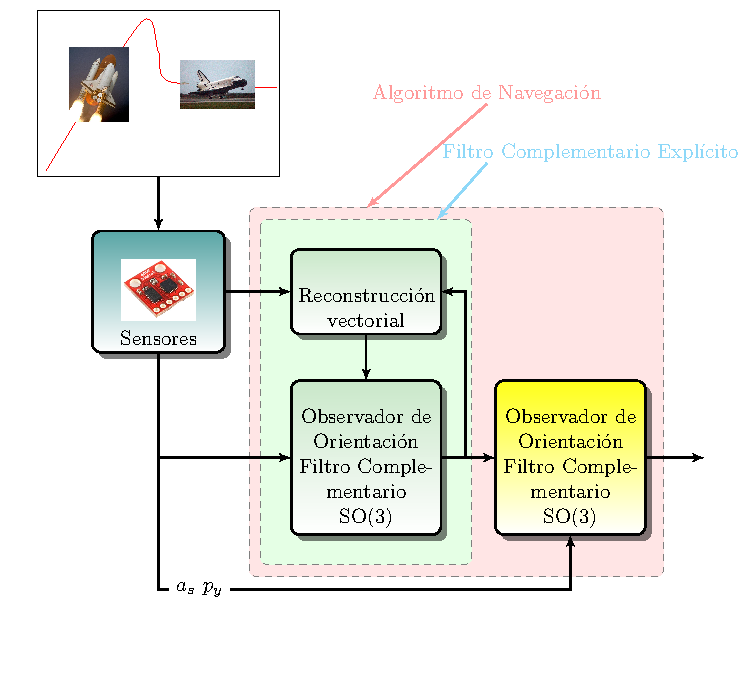
\includegraphics[width=9cm,clip]{intro_fig4.pdf}
\caption{Esquema simplificado del algoritmo de Mahony-Scandaroli.}
\scriptsize{Tell us about.}
\label{solucionMS_fig1}
\end{center}
\end{figure}
La solución de este problema, desde el enfoque de Mahony-Scandaroli, deriva en el algoritmo de navegación de filtros complementarios en SO(3) en cascada, esquematizado en el diagrama de bloques de la Figura \ref{solucionMS_fig1}. 
%%%%%%%%%%%%%%%%Corrección 5 de mayo 2015
Este propone la combinación en cascada de dos observadores del tipo filtro complementario en SO(3): el observador de orientación y el observador de posición. Bajo este esquema, el observador orientación utiliza la medición de la velocidad angular $\Omega_s$ \footnote{ Elemento de conjunto de \emph{información sensorial disponible} $S$} y la matriz de rotación $R_y$, donde esta última proviene de una fórmula de  reconstrucción vectorial que conjuga la medición de valores vectoriales en $\marco{B}$ ($v_i$)\footnote{No confundir con la notación, detallada más adelante, de la velocidad lineal del cuerpo $\hat{v}$ y la incertidumbre del modelo de medición $\hat{v}_k$.}, sus valores teóricos en el $\marco{A}$ ($v_{i,0}$), y el punto de estabilidad encontrado por el observador de orientación para la matriz de rotación ($\hat{R}$, estos relacionados en la siguiente ecuación, que toma en cuenta $n$ mediciones vectoriales).
\begin{equation}\label{ReconstruccionVectorial}
R_y=\sum_{i=1}^{n}(v_{i,0})_\times\hat{R}(v_i)_\times
\end{equation}
Se considera $(\cdot)_\times$ el operador "retorcedor" (screw), reportado en \cite{Mahony2008}
%%%%%
El observador de orientación usando la reconstrucción vectorial y la medición de la velocidad angular, determina:
\begin{itemize}
\item $\hat{\Theta}$: La estimacion de la orientación en términos de los ángulos de Euler .
\item  $\hat{\Omega}$: La estimacion(corrección) de la velocidad angular en $\marco{B}$, donde $\marco{B}$ denota un marco referencial cartesiano fijo al cuerpo desde donde se realiza la medición de la aceleración y velocidad angular.
\item $\tilde{R}$: El error de estimación de la matriz de rotación, definida a través de la matriz de transformación $\marco{E}\hookrightarrow\marco{B}$, donde $\marco{E}$ denota el marco referencial de estimación, el cual teóricamente converge hacia $\marco{B}$ y se considera el resultado de la estimación de $\marco{B}$ por el observador de orientación .
\item $\hat{R}$: La estimación de la matriz de rotación, definida como la matriz de transformación $ \marco{E}\hookrightarrow\marco{A}$,  donde $\marco{A}$ denota el marco referencial inercial, con direccion y origen fijos en un punto sobre la tierra.
\end{itemize}
Siguiendo el esquema del Mahony-Scandarolli, en cascada el observador de posición tipo Filtro complementario en SO(3), toma el resto de las variables incluidas en $S$ (la medición de la aceleración $a_s$ y la medición de la posición $p_y$), junto con las matrices de transformación determinadas por el anterior observador, para obtener:
\begin{itemize}
\item $\hat{p}$: La estimación de la posición en $\marco{A}$.
\item $\hat{v}$: La estimación de la velocidad en $\marco{A}$.
\end{itemize}
Finalmente, los dos grupos de variables estimadas por ambos observadores conforman la \emph{estimación de la información de navegación}, que puede ser denotada por el vector columna $X=[\hat{p}~\hat{v}~\hat{\Theta}~\hat{\Omega}]$.\par

%En resumen, el enfoque original del algoritmo de observadores en cascada de Mahony-Scandaroli, resuelve la determinación de la información de navegación en tres niveles de procesamiento:
%a) la reconstrucción vectorial de la matriz de rotación $R_y$ usando la medición de un acelerómetro $a_s$ y un magnetómetro $m_s$\footnote{El desarrollo teórico y práctico de Mahony en \cite{Mahony2008} demuestra que no es absolutamente necesario incluir ambas mediciones. Y si el caso fuese de que alguna de las señales es demasiado ruidosa se puede prescindir de la misma.}; b) la determinación de la estimación de la velocidad angular $\hat{\Omega}$, la estimación de la orientación en términos de los ángulos de Euler $\hat{\Theta}$, y la estimación de la matriz de rotación $\hat{R}$ con su respectivo error $\tilde{R}$\footnote{Definida como $\tilde{R}=R_y\hat{R}^T$}, los que se determinan usando las señales de la reconstrucción vectorial y la medición de un giroscopio $\Omega_s$; c) la determinación de la estimación de la posición $\hat{p}$, y la velocidad lineal $\hat{v}$ a partir de las anteriores salidas, es decir $\tilde{R}$ y $\hat{R}$, junto con la medición de posición $p_y$ y la aceleración $a_s$.\par
%%
Como señala Mahony, la principal desventaja en la formulación de los filtros complementarios pasivo y directo es la sensibilidad a la matriz de entrada $R_y$. Esta matriz es usada en el mapeo de la medición de la velocidad angular al marco inercial $\marco{A}$, y por esta razón, la determinación de esta matriz juega un papel central en el desempeño final del sistema. Considerando esto la determinación desde el enfoque de la reconstrucción vectorial de Mahony-Scandarolli es una solución sub-óptima a el problema de optimización del cálculo de la matriz de rotación, el cual indica que: \emph{a partir de la medición de cantidades vectoriales conocidas respecto a $\marco{B}$, la matriz de rotación puede ser determinada en el argumento que minimiza la función de coste definida como:}
\begin{equation}\label{ProblemaOptimizacion}
R^*=\arg~\min_{R}\left\{\sum_i|v_{0,i}-Rv_{m,i}|^2\right\}
\end{equation}
Donde, la matriz de rotación óptima $R^*$ es obtenida en el argumento que minimiza la función de coste compuesta por la suma de los cuadrados de los módulos de la diferencia de: los valores de las mediciones vectoriales rotadas al marco inercial (R$v_{m,i}$), respecto a los valores teóricos conocidos de dichas cantidades vectoriales ($v_{0,i}$)\footnote{Donde los sub-índices corresponden a las distintos valores vectoriales medibles.}.
La relación sub-optima se establece en la incorporación del estimado de la matriz de rotación $\hat{R}$ como la resolucción de la ecuación de Lyapunov, asumiendo esta última como solución a \label{ProblemaOptimizacion}. Se asume inicialmente, que este hecho incorpora una sensibilidad extra: a ruidos de medición, sesgos de medición y los estados transitorios de ascentamiento, reduciendo en gran medida el desepeño del algoritmo de navegación en general. 
%%%%%%%%%%%%%%
%%%%%%%%%%%%%%
%%%%%%%%%%%%%%
\section{Reconstrucción Óptima de la matriz de rotación}
%%
Considerando las desventajas señaladas en la sección anterior, se indentifica que el mejorar la reconstrucción de la matriz de rotación puede traer mejoras en en el desempeño general del algoritmo. Para ello, se buscará solucionar de manera óptima el problema de determinación de la matriz de rotación\footnote{Planteado en la referencia \cite{Mahony2008}} a partir de mediciones vectoriales.
%%%%%%%%%%%%%%
%%%%%%%%%%%%%%
%%%%%%%%%%%%%%
\subsection{Determinación óptima de la matriz de rotación a partir del modelo de medición del vector gravitacional en cuaterniones.}
\begin{figure} [t]
\begin{center}
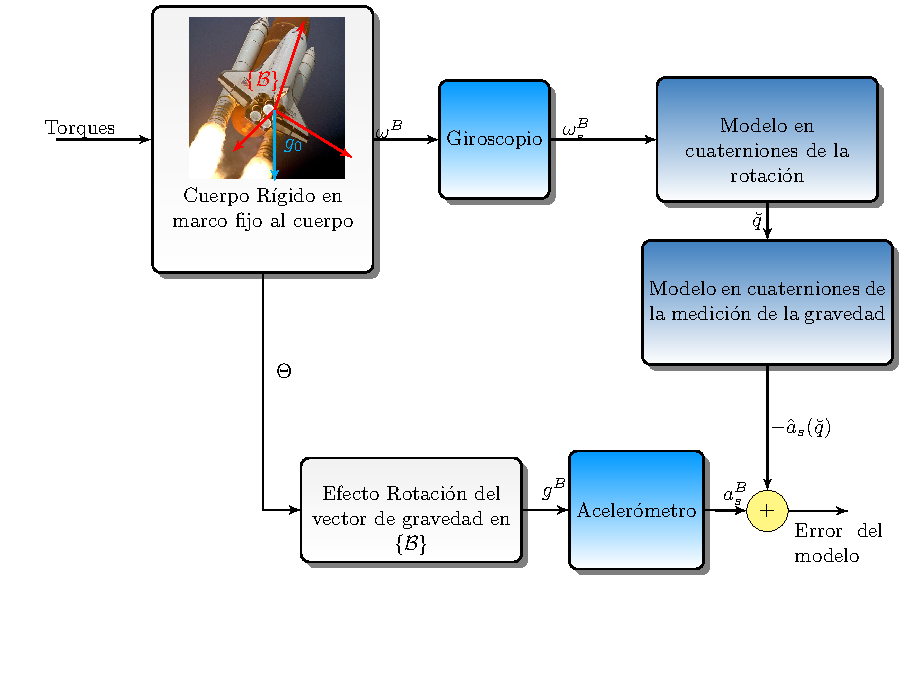
\includegraphics[scale=0.50,viewport=20 50 430 330,clip]{ObsOptimo_fig3.pdf}
\caption{Caracterización del error del modelo de medición.}
\label{ObsOptimo_fig2}
\end{center}
\end{figure}
%%
Se propone la determinación de la matriz de rotación interpretando el fenómeno de inclinación de campo gravitacional respecto al marco $\marco{B}$ con un observador óptimo en cuaterniones. En donde, el observador se consititutye en el esquema detallado en la figura \ref{ObsOptimo_fig2}. En este equema, se considera el fenómeno de rotación de un cuerpo rígido (excitado por \emph{torques} desconocidos) descrito por dos variables: la orientación y su velocidad angular, representadas por las salidas $\Theta$ y $\Omega$, respectivamente, estos parámetros son medidos:
\begin{enumerate} 
\item La velocidad angular por un giroscopio, obteniendo $\Omega_s$.
\item La orientación $\Theta$ de manera indirecta por un acelerómetro, el cual mide inclinación del vector gravitacional respecto al marco fijo al cuerpo $\marco{B}$
\end{enumerate}
En este arreglo, el observador incorpora correcciones sistemáticas al modelo de cinemático de rotación en términos del cuaternión unitario, que se calculan a partir de:
\begin{itemize}
\item El error del modelo de medición de la aceleración gravitacional 
\item Y la medición de la velocidad angular $\Omega_s$.
\end{itemize}
De manera tal que se reduce el error del modelo de medición, ajustando así el cuaternión que rota el valor teórico de la gravedad en el marco referencial inercial ($[0,0,g_0]^T$), alineando el mismo a la medición vectorial $a_s$.\par
%%
Esto último es posible, dado que el cuaternión se define en las rotaciones de los ángulos de Euler (ver \cite{Altmann1986}).\par
%%%
\subsection{Observador óptimo en cuaterniones}
En la definición del observador óptimo, se identifica entonces el caso particular de la ecuación \ref{ProblemaOptimizacion}, donde la matriz de rotación óptima $R^*$ depende de la relación de optimización del cuaternión unitario de rotación $\breve{q}$, denotado por $\breve{q}=q_0+q_1i+q_2j+q_3k$ en $\mathbb{Q}:\mathbb{R}\times\mathbb{C}^3$:
\begin{equation}\label{ProblemaOptimizacionAcc}
R^*(\breve{q})=R\left(q^*=\arg\min_{\breve{q}}\left\{a_s-R^T(\breve{q})g_0\right\}\right)
\end{equation} 
De esa manera, la solución a la matriz de rotación óptima deriva del procedimiento  de optimización del cuaternión unitario que rota el valor teórico de la gravedad $g_0$ hacia la medición de la inclinación campo vectorial gravitatorio $a_s$, en la relación que establece $\hat{a}_s$ en la siguiente ecuación, como la estimación de la medición vectorial de la gravedad en función del cuaternión unitario \cite{Sola2012}:
\begin{equation}\label{chap2:ModeloMedicion}
\hat{a}_s=\bar{\breve{q}}\otimes\breve{g_0}\otimes\breve{q}=Rg_0=g_0\begin{bmatrix}2(q_1q_3-q_oq_2)\\2(q_2q_3+q_0q_1)\\q_0^2-q_1^2-q_2^2-q_3^2\end{bmatrix}
\end{equation}
La evolución en el tiempo del cuaternión unitario esta delimitado en la descripción cinemática del movimiento rotación en $\mathbb{Q}$, definida como:
%%%
\begin{equation}\label{modelo2}
\dot{\breve{q}}=\frac{1}{2}\breve{q}\otimes\breve{\Omega}
\end{equation}
Donde, la derivada del cuaternión unitario se define en el producto de cuaterniones \footnote{Denotada por el símbolo $\otimes$} de la velocidad angular en $\mathbb{Q}$\footnote{Definida como un cuaternión puro, en donde la parte real es cero, y las componentes están repartidas en $i$, $j$ y $k$, para la velocidad angular en los ejes $x$, $y$ y $z$, respectivamente} ($\breve{\Omega}$) y el cuaternión unitario ($\breve{q}$).\par
A partir de esto, el reto asumido por el observador es determinar el cuaternión óptimo en el tiempo $T$, conciderando de tres elementos: i) la incertidumbre en las condiciones iniciales $\tilde{q}_0$ y $\hat{v}_0$, ii) la incertidumbre del modelo discretizado del proceso de rotación del cuaternión $\hat{w}_k$, definido en (\ref{quaMod}), donde $f^0_k$ es la versión discretizada de (\ref{modelo2}) y $\hat{\breve{q}}_{k}$ es el estimado discreto del cuaternión.
\begin{equation}
\label{quaMod}
\hat{\breve{q}}_{k+1}=f^0_k(\hat{\breve{q}}_k,\Omega_k)+\hat{w}_k
\end{equation}
 iii) Y la incertidumbre en la estimación de la medición vectorial de la gravedad, el cual se define como la resta del valor estimado $\hat{a}_{s,k}$ con señal proveniente del acelerómetro $a_{s,k}$ en el tiempo $k$,
\begin{equation}
\hat{v}_k=a_{s,k}-\underbrace{\hat{a}_{s,k}}_{\hat{a}_{s,k}=h_k(\hat{\breve{q}}_k)}
\end{equation}
A partir de esto, la función objetivo desde el punto de vista del observador se deduce como la adición de dos normas específicas
\begin{equation}
q^*_k=\arg~\min_{q_k}\left\{norm_0(\tilde{q}_0,\hat{v}_0)+\sum^k_{i=0}norm_1(w_i,v_i)\right\}
\end{equation}
La primera combina la incertidumbre de condiciones iniciales de medición $\hat{v}_0$ y estado inicial del cuaternión unitario $\tilde{q}_0$ y la segunda combina la evolución en el tiempo de la incertidumbre del modelo $\hat{w}_k$ y de medición $\hat{v}_k$, ambos para el invervalo de  tiempo discreto $i\in\{k_0,...,k_f\}$. El problema se mantiene en la búsqueda del estimado $\hat{\breve{q}}_{k+1}$ haciendo correcciones sucesivas sobre la incertidumbre del modelo $\hat{w}_k$.\par
La solución propuesta a este problema hace uso de Programación Dinámica (PD) \cite{Lewis2012} en la versión lineal del modelo del proceso de rotación del cuaternión (\ref{quaMod}) y del modelo de la medición.
\begin{gather}
\hat{w}_{k}=-\underbrace{P_kH_k^T(R+H_kP_kH_k^T)}_K\tilde{y}_k\\
\hat{w}_k^TF^{-T}P_kA^{-1}\hat{w}_k=\hat{w}_k^T(F^{-T}QF^{-1}+P_k-KH_kP_k)\hat{w}_k
\end{gather}
Lo que establece el estimador de estimador lineal en:
\begin{equation}\label{chap2:ObservadorLineal}
\hat{\breve{q}}_{k+1}=F\hat{\breve{q}}_k+B\Omega_{s,k}+K(y_k-H\hat{x}_k)
\end{equation}
%%%%%%%%%%%%%%%
%%%%%%%%%%%%%%%%
%%%%%%%%%%%%%%%%%
\section{Metodología de la evaluación experimental}\label{Metodologia}
El abordaje experimental trata de probar que la inclusión de un Observador Óptimo  para reconstrucción de la matriz de rotación en el esquema del algoritmo de navegación compuesto por los filtros complementarios en SO(3), incorporía mejoras en la estimación total de la información de navegación. Para ello, se realizan experimentos orientados a comparar el algoritmo original y el algoritmo modificado. en las mismas condiciones de operación. Bajo esta premisa, los experimentos son conducidos de tal forma que ambos algoritmo procesan la misma información de entrada, que proviene de los mismos  sensores de navegación: un módulo receptor GPS MTK-2309; un acelerómetro MEMS de bajo costo ADXL330 de $\pm3g$ y tres grados de libertad; y los giroscopios MEMS IDG500 y LPY330AH, que miden las velocidades angulares en las direcciones de los versores del marco $\marco{B}$. \par
%%
De esa manera, los experimientos son realizados separando los casos de estudio en dos plataformas distintas para: 
\begin{enumerate}
\item El estudio de la estimación de los ángulos de Euler en una componente para movimientos de hasta $1[rad/s]$.
\item El estudio de las capacidades de estimación de la posición y velocidad linea en tres dimensiones para un circuito cerrado recorrido en un automóvil.
\end{enumerate}
\subsection{Plataforma experimental de la estimación de los ángulos de Euler}\label{Plataforma2}
\begin{figure}
\centering
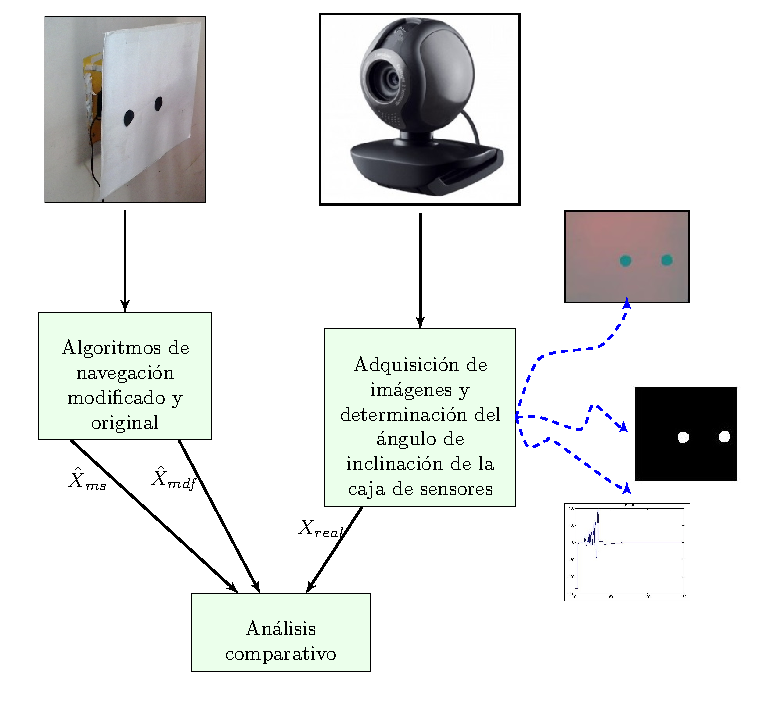
\includegraphics[width=26.5em]{plataforma_fig13.pdf}
\caption{Esquema general de la plataforma experimental evaluativa.}
\scriptsize{Fuente: Elaboración Propia}
\label{plataforma_fig10}
\end{figure}
La plataforma experimental de la estimación de los ángulos de Euler fue implementada siguiendo el esquema de la Figura \ref{plataforma_fig10}, donde un arreglo de marcas negras en una plancha blanca sujeta a la caja de sensores permite hacer el seguimiento de la evolución del movimiento angular de referencia $X_{real}$, en forma simultánea a la captura de las señales de los sensores de navegación. De esa manera, los algoritmos de navegación determinan la estimación de la información de navegación $\hat{X}_{mdf}$ y $\hat{X}_{mh}$; y de forma paralela haciendo seguimiento con una cámara se determina el valor angular de referencia correspondiente a la evolución temporal de la componente de los ángulos de Euler, sobre la cual se está haciendo el análisis. Bajo estas condiciones se hacen tres arreglos distintos para los tres ejes del $\marco{B}$, es decir en $x$ para $\phi$, en $y$ para $\theta$, y en $z$ para $\psi$, analizando cada ángulo por separado.
%%%%%%%%%%%%%%%%%%%%%%%%%%%
%%%%%%%%%%%%%%%%%%%%%%%%%%%
\subsection{Plataforma experimental de la estimación de la posición y velocidad lineal}
Para la evaluación de la estimación de la posición y velocidad lineal el esquema implementado utiliza como como referencia la información de un módulo comercial de localización GPS Etrex-Garmin que tiene una precisión de hasta 2 metros, por mucho mayor a la del módulo GPS usado dentro del conjunto de sensores de navegación, esto gracias a la ganancia de su antena que le permite capturar un mayor número de satélites, además de tener una memoria especializada para la captura de datos de Efemérides y Calendarios pasados. Este dispositivo cuenta con un altímetro y una brújula electrónica, mejorando su precisión aún más.\par%%
\begin{figure}
\centering
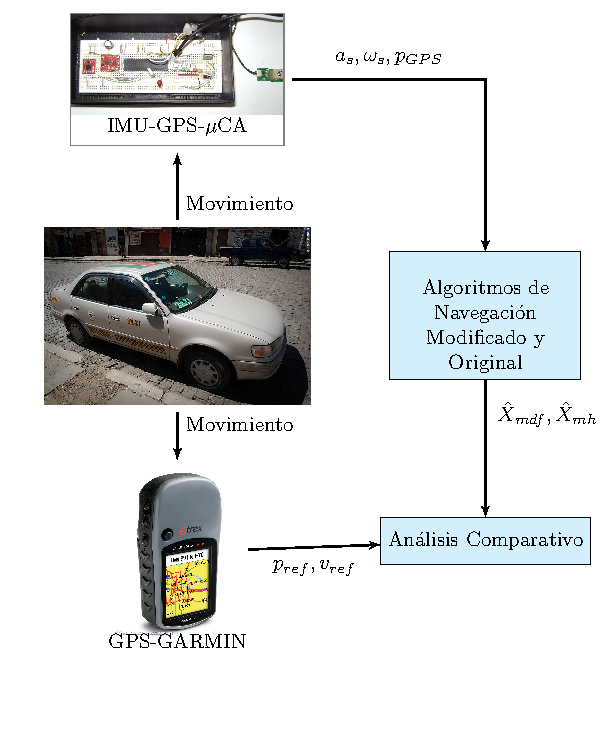
\includegraphics[width=22.5em]{plataforma_fig14.pdf}
\caption{Plataforma experimental de la estimación del movimiento lineal.}
\scriptsize{Fuente: Elaboración Propia}
\label{plataforma_fig9}
\end{figure}
Los experimentos son realizados siguiendo circuitos cerrados en un vehículo en donde se monta una caja que contiene al sensor comercial y los sensores de navegación de forma tal que es posible realizar la estimación de la información de navegación y capturar información de referencia. De forma similar al caso del movimiento angular, como se describe en la figura \ref{plataforma_fig9}, la información de los sensores de navegación es procesada por los algoritmos de navegación obteniendo $\hat{X}_{mh}$ y $\hat{X}_{mdf}$; y de forma simultanea, durante el movimiento del vehículo, se captura la información de referencia que corresponde al GPS GARMIN-ETEX.

\section{Resultados experimentales}
En esta sección se presentan los resultados experimentales resaltando sus principales caracterísiticas.
\subsection{Prueba con la plataforma experimental de la estimación los ángulos de Euler}
Esta fase emplea el esquema experimental descrito en la sección \ref{Plataforma2}, en la cual el sensor angular de video (constituido por una cámara) captura la información de la rotación de uno de los ángulos de Euler, al mismo tiempo que los algoritmos de navegación realizan la estimación de la misma variable\footnote{Dentro del conjunto de datos que conforman la información de navegación estimada.}.\par
%%%
Los resultados obtenidos de uno de los varios ensayos realizados para la comparación del desempeño de la estimación la orientación se muestran en las gráficas de la Figura \ref{PlotPh1}, donde la señal de color azul corresponde a la estimación, la de color verde para el  algoritmo original, y de color rojo para la referencia. Las graficas se ordenan mostrando los resultados de la estimación para los ángulos $\phi$, $\theta$ y $\psi$, ordenados de arriba hacia abajo en el orden en que se los menciona.\par
%%
En el primer caso, el movimiento inicia en -2º y termina en poco menos de -3º y los ángulos de rodadura y guiñeo se mantienen en 0º, en velocidades  de hasta 17º/s. Para la estimación con el algoritmo modificado los errores oscilan entre $9.04E-4º$ y $10.58º$ en contraste a los $7.33E-3º$ a $18.97º$\footnote{Estos valores están en valor absoluto respecto a la señal original.} para el algoritmo original. 
En estas gráficas los errores cometidos por el algoritmo original son mucho mayores a los del algoritmo modificado, donde este último gana definitivamente a partir de 15 segundos.\par
\begin{figure}
\begin{center}
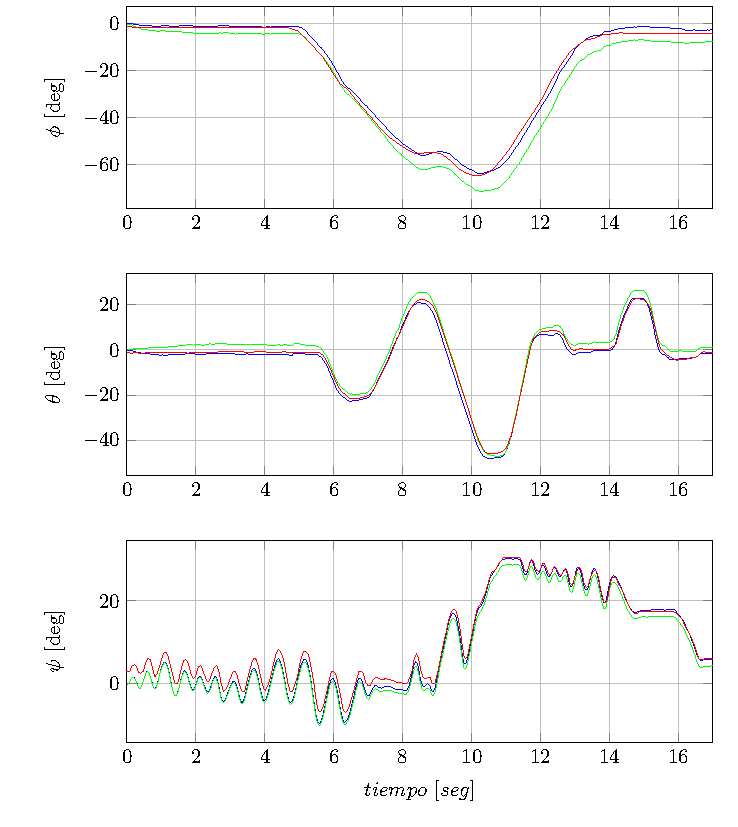
\includegraphics[width=26em]{PlotAngles1.pdf}
\caption{Prueba comparativa de la estimación de los ángulos de Euler. }
\label{PlotPh1}
\scriptsize{Los ángulos de euler, se denotan en el vector columna $\Theta=[\phi~\theta~\psi]^T$, con $\phi$ para el alabeo, $\theta$ para la rodadura y $\psi$ para el guiñeo.}
\end{center}
\end{figure}
En el segundo caso, los movimientos están limitados dentro de la banda de $\pm45[º/s]$. En este ensayo, el desempeño del algoritmo modificado mejora sobre al algoritmo original, y a partir de los 13 segundos la convergencia del método modificado es insuperable\par
%%
Por último, para el tercer caso, los ensayos fueron realizados con la plataforma en posición horizontal dando al sistema mayor movilidad. Con estas características, generan trayectorias de cambios abruptos. Se hace importante mencionar que en estas condiciones el vector gravitacional está apuntando paralelo al eje de rotación, dificultando la estimación vectorial y así la estimación del ángulo de guiñeo para el algoritmo original; por esta razón la capacidad de convergencia del método original, cuando la condición inicial del ángulo muy distinta de cero, se ve afectada considerablemente. Para este ensayo el ángulo inicial de guiñeo es de 5º, lo que permite ver el efecto anteriormente mencionado, donde a pesar de que las condiciones iniciales de error en los ángulos de Euler no son nulas, el algoritmo modificado reduce progresivamente el error, en contraste con el algoritmo original, el cual permanece con un error constante de 1.5º, por lo menos durante toda la ventana temporal que dura el experimento.\par
%%%%%%%%%%%%%%%%
%%%%%%%%%%%%%%%%
%%%%%%%%%%%%%%%%
\subsection{Prueba con la plataforma experimental de la estimación del movimiento lineal}
Los experimentos realizados con esta plataforma permiten ver el desempeño del algoritmo para estimar el movimiento lineal, es decir la velocidad lineal y la posición en el tiempo. \par
%\begin{figure}
%\begin{center}
%\includegraphics[width=25em]
%{pruebas_fig1a.jpg}
%\caption{Circuito cerrado \scriptsize{Fuente: Google Earth y DigitalGlobe 2013}}
%\label{pruebas_fig1}
%\end{center}
%\end{figure}
Los ensayos para la evaluación de la estimación del movimiento lineal se desarrollan en un circuito cerrado en una ruta que tiene una longitud de $1.53[Km]$, pasa por calles con buena línea de vista, sin muchos árboles ni edificios.
%%
\begin{figure}
\begin{center}
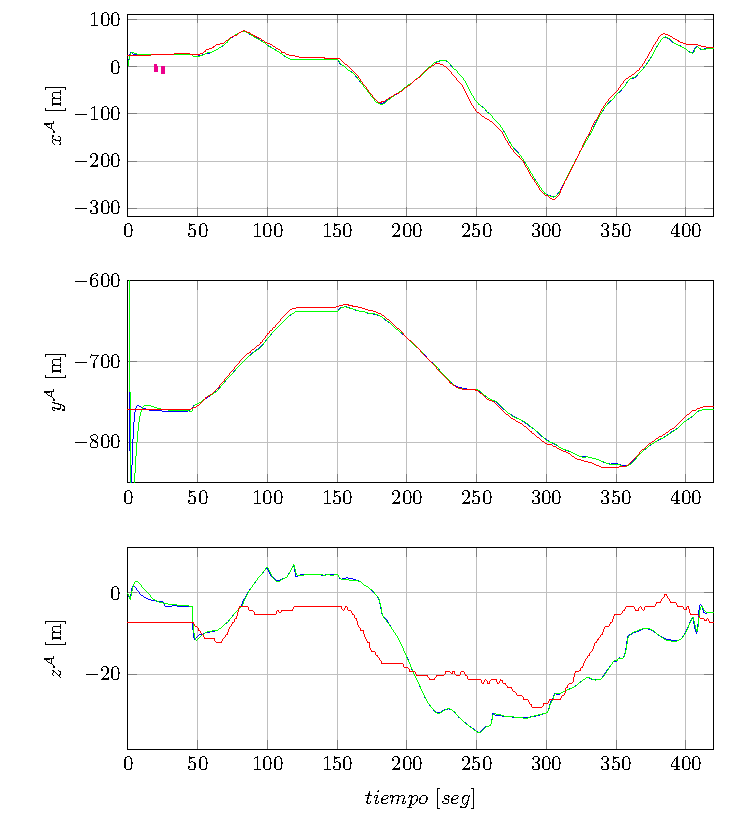
\includegraphics[width=25em]
{PlotPosition1.pdf}
\caption{Resultados de la estimación de la posición.}
\scriptsize{Resultados de la estimación de con datos simulados. Resultados típicos del repetidos intentos.}
\label{PlotX1}
\end{center}
\end{figure}
%%
En todas las gráficas, los resultados de la estimación del algoritmo Original son representados en la línea de color verde, para la estimación del algoritmo modificado de color azul, y para la señal de referencia en una línea de color rojo.
%%
Las pruebas de estimación de la posición muestran errores, despues de la etapa transitoria que varia entre 2[m] y 10[m]. Respecto al movimiento horizontal, los errores verticales muestran un mala calidad, sin embargo hay que considerar que los errores en la altitud son  típicamente son grandes \footnote{Esto no pone en cuestión la veracidad de la información entregada por el GPS-Garmin, debido a que este dispositivo utiliza la información de un barómetro, que sin duda tiene mejor precisión.} en navegación GPS. A pesar de eso, es de consideración ver que la información estimada se aproxima a la señal de referencia, mucho más que la medición del sensor de navegación GPS-MTK3329. \par
%%
En esta prueba con respecto a la estimación de la velocidad, dado que la velocidad de referencia esta expresada en $\marco{A}$ la matriz de rotación juega un papel fundamental en la estimación para hacer la transformación correspondiente. Entonces, esto sugiere que la convergencia está delimitada por la capacidad de los algoritmos para estimar los ángulos de Euler. Los resultados de las pruebas realizadas son mostrados en la Figura \ref{PlotU1}, en la que se muestra las velocidades en $x$, $y$ y $z$ del marco referencial inercial $\marco{A}$ con la misma notación de colores que se ha venido manteniendo desde la Figura \ref{PlotPh1}.\par
\begin{figure}
\begin{center}
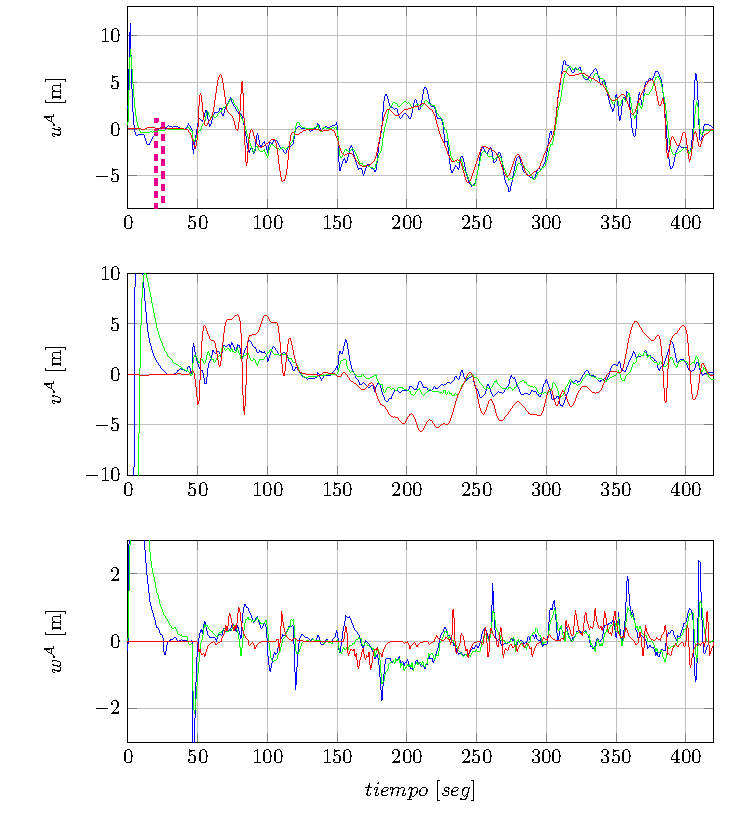
\includegraphics[width=25em]
{PlotVelocity1.pdf}
\caption{Velocidad lineal en el eje X.}
\scriptsize{Resultados de la estimación de con datos simulados. Resultados típicos del repetidos intentos.}
\label{PlotU1}
\end{center}
\end{figure}
%%%
\subsection{Análisis Comparativo}
En la Tabla \ref{resultados_tb1} se ordenan los errores absotulos promedio (EAP) y las diferencias porcentuales para cada variable.\par
% An example of a floating table. Note that, for IEEE style tables, the 
% \caption command should come BEFORE the table. Table text will default to
% \footnotesize as IEEE normally uses this smaller font for tables.
% The \label must come after \caption as always.
%
%\begin{table}[!t]
%% increase table row spacing, adjust to taste
%\renewcommand{\arraystretch}{1.3}
% if using array.sty, it might be a good idea to tweak the value of
% \extrarowheight as needed to properly center the text within the cells
%\caption{An Example of a Table}
%\label{table_example}
%\centering
%% Some packages, such as MDW tools, offer better commands for making tables
%% than the plain LaTeX2e tabular which is used here.
%\begin{tabular}{|c||c|}
%\hline
%One & Two\\
%\hline
%Three & Four\\
%\hline
%\end{tabular}
%\end{table}
\begin{table}[!t]
\caption{Tabla comparativa del desempeño de Algoritmo de tres observadores en cascada y el de Mahony-Scandaroli.}
\label{resultados_tb1}
\begin{center}\scriptsize
\begin{tabular}{|p{0.6in}|p{0.7in}|p{0.7in}|p{0.7in}|} \hline
\textbf{Variable estimada}&\textbf{EAP del algoritmo modificado}&\textbf{EAP del algoritmo original}&\textbf{Diferencia Porcentual del Algoritmo Modificado respecto al Original.} \\ \hline
%--------------------------------------------------------------------->
Posición en el eje X ($x$) &5.8862[m]&5.9427[m]&0.9596\%\\ \hline
Posición en el eje Y ($y$) &3.5445[m]&4.7739[m]&34.6828\%\\ \hline
Posición en el eje Z ($z$)&6.1698[m]&6.3369[m]&2.7080\%\\ \hline
Velocidad lineal en el eje X ($v_x$) &0.8214[m/s]&0.7871[m/s]&{-12.1305\%}\\ \hline
Velocidad lineal en el eje Y ($v_y)$&3.1564[m/s]&3.3291[m/s]&5.4710\%\\ \hline
Velocidad lineal en el eje Z ($v_z$)&0.4445[m/s]&0.5697[m/s]&28.1664\%\\ \hline
Ángulo de alabeo ($\phi$ )&1.3579[Deg]&3.7560[Deg]&177.97\%\\ \hline
Ángulo de rodadura ($\theta$ )&1.4635[Deg]&2.801[Deg]&91.394\%\\ \hline
Ángulo de guiñeo ($\psi$ )&1.3268[Deg]&2.1855[Deg]&44.53\%\\ \hline
\end{tabular}
\end{center}
\end{table}
En esta tabla se puede ver globalmente que el algoritmo modificado es superior en casi todas las variables, lo que se corrobora con el cálculo de la diferencia porcentual promedio (DPP) igual a 40.92\%, es decir que en promedio se tiene 40.92\% mejor desempeño en la estimación de la información de navegación para el algoritmo modificado respecto al original.\par
%%
Analizando los pares de EAP mostrados en la Tabla \ref{resultados_tb1} vemos una marcada tendencia que indica que el algoritmo modificado supera al algoritmo original. Dentro de las diferencias más relevantes se tienen: la estimación de la posición en el eje $y$  con $1.22[m]$ de distancia en promedio, y los ángulos de alabeo y rodadura, con $2.39º$ y $1.73º$, respectivamente.
\subsection{Tiempos de Procesamiento.}
%%
En relación a los tiempos de procesamiento se mide el tiempo de procesamiento conjunto de $2,957$ puntos de muestreo, es decir para $49.4311 [s]$ de tiempo de estimación. En cada iteración el tiempo de procesamiento es de $1.0158[ms]$ para el algoritmo modificado y $0.7954 [ms]$ para el algoritmo original, definiendo una diferencia porcentual promedio de:
\begin{equation}
DPP_{\texttt{tiempo de procesamiento}}=-21.6933\%
\end{equation}
Lo que indica que el algoritmo original utiliza $21.6933\%$ menos tiempo que el algoritmo modificado.
%\section{Análisis y discusión de los resultados.}
%La convergencia para la estimación de la orientación del método propuesto en el presente trabajo se verifica con el análisis visual de las gráficas de la Figura \ref{PlotPh1}. En general, las aproximaciones son bastante cercanas y alcanzan la referencia definitivamente a partir de los doce segundos reduciendo el error. Esto marca una indicación positiva para la inclusión del observador óptimo en la estructura de los filtros complementarios en $SO(3)$.\par
%%%
%Respecto a la estimación del movimiento lineal, los resultados no son del todo alentadores. En algunos casos el error puede llegar hasta $20[m]$, con un promedio de $5.2[m]$ y en los mejores casos se mantiene dentro de los dos metros de error. Esto reduce en gran medida el rango de aplicaciones del algoritmo, así como está planteado. Y deja la imperante necesidad de incorporar un segundo método de estimación en la determinación de la posición, por ejemplo, como el reportado en \cite{Merwe2004}. A pesar de este comportamiento, la estimación de la velocidad permite pensar en aplicaciones de control en aeronaves no tripuladas (Unmanned Aircraft Vehicles, UAVs).\par
%Refiriéndonos a los errores de la posición en los ejes X y Y de la Figura \ref{resultados_tb1}, se acerca mucho al error típico del GPS usado \cite{Mediatek2009} cuyo valor es de 5m en 2D comparado al 4.71 [m], y seguramente en mejores condiciones de visibilidad\footnote{Que típicamente se encuentran en las zonas abiertas en las que los UAV aplicados a vigilancia o exploración funcionan.} el algoritmo promediaría mejores condiciones de estimación.\par
%%% 
%%%
%Según estos datos, el algoritmo modificado es capaz de computar las trayectorias con tan buena precisión como tenga nuestro sensor de posición. Sin embargo el tema de alineación inicial es vital para tener una buena estimación, a pesar de que esto no afecta la estabilidad del sistema en ninguna escala.


% An example of a floating figure using the graphicx package.
% Note that \label must occur AFTER (or within) \caption.
% For figures, \caption should occur after the \includegraphics.
% Note that IEEEtran v1.7 and later has special internal code that
% is designed to preserve the operation of \label within \caption
% even when the captionsoff option is in effect. However, because
% of issues like this, it may be the safest practice to put all your
% \label just after \caption rather than within \caption{}.
%
% Reminder: the "draftcls" or "draftclsnofoot", not "draft", class
% option should be used if it is desired that the figures are to be
% displayed while in draft mode.
%
%\begin{figure}[!t]
%\centering
%\includegraphics[width=2.5in]{myfigure}
% where an .eps filename suffix will be assumed under latex, 
% and a .pdf suffix will be assumed for pdflatex; or what has been declared
% via \DeclareGraphicsExtensions.
%\caption{Simulation Results}
%\label{fig_sim}
%\end{figure}

% Note that IEEE typically puts floats only at the top, even when this
% results in a large percentage of a column being occupied by floats.


% An example of a double column floating figure using two subfigures.
% (The subfig.sty package must be loaded for this to work.)
% The subfigure \label commands are set within each subfloat command, the
% \label for the overall figure must come after \caption.
% \hfil must be used as a separator to get equal spacing.
% The subfigure.sty package works much the same way, except \subfigure is
% used instead of \subfloat.
%
%\begin{figure*}[!t]
%\centerline{\subfloat[Case I]\includegraphics[width=2.5in]{subfigcase1}%
%\label{fig_first_case}}
%\hfil
%\subfloat[Case II]{\includegraphics[width=2.5in]{subfigcase2}%
%\label{fig_second_case}}}
%\caption{Simulation results}
%\label{fig_sim}
%\end{figure*}
%
% Note that often IEEE papers with subfigures do not employ subfigure
% captions (using the optional argument to \subfloat), but instead will
% reference/describe all of them (a), (b), etc., within the main caption.





% Note that IEEE does not put floats in the very first column - or typically
% anywhere on the first page for that matter. Also, in-text middle ("here")
% positioning is not used. Most IEEE journals/conferences use top floats
% exclusively. Note that, LaTeX2e, unlike IEEE journals/conferences, places
% footnotes above bottom floats. This can be corrected via the \fnbelowfloat
% command of the stfloats package.



\section{Conclusion}

En este trabajo se ha desarrollado una arquitectura en cascada de observadores basados en el análisis funcional de sus entradas y salidas. En esta se consideran como fuente de información a las señales de una IMU y un módulo receptor GPS. Se realizaron las pruebas experimentales en diferentes arreglos de la plataforma experimental de la estimación de los ángulos de Euler, que permitieron realizar la comparación de la estimación respecto a una señal de referencia. De manera global, se logra diseñar e implementar un sistema de navegación de procesamiento fuera de línea para los datos de una IMU y un GPS, el cual puede estimar la orientación y la posición con seis grados de libertad de cualquier cuerpo rígido. Además se propone un algoritmo de navegación que incorpora una variación de los métodos de Mahony-Scandaroli. Este algoritmo está constituido en tres etapas de observación: la primera con un observador de la orientación EKF basado en cuaterniones para la reconstrucción de la matriz de rotación, la segunda con un filtro complementario en $SO(3)$ de orientación, y la tercera con el observador de posición.
\par
%%
Basado en los resultados de la experimentación se puede decir que el algoritmo de navegación implementado tiene una ventaja considerable respecto al anterior método. Y aunque incrementa la complejidad final del algoritmo, no es una limitante para la implementación en algún procesador digital con capacidad de procesamiento suficiente.\par
% conference papers do not normally have an appendix


% use section* for acknowledgement
\section*{Acknowledgment}
The authors would like to thank...
% trigger a \newpage just before the given reference
% number - used to balance the columns on the last page
% adjust value as needed - may need to be readjusted if
% the document is modified later
%\IEEEtriggeratref{8}
% The "triggered" command can be changed if desired:
%\IEEEtriggercmd{\enlargethispage{-5in}}

% references section

% can use a bibliography generated by BibTeX as a .bbl file
% BibTeX documentation can be easily obtained at:
% http://www.ctan.org/tex-archive/biblio/bibtex/contrib/doc/
% The IEEEtran BibTeX style support page is at:
% http://www.michaelshell.org/tex/ieeetran/bibtex/
\bibliographystyle{IEEEtran}
% argument is your BibTeX string definitions and bibliography database(s)
\bibliography{IEEEabrv,BiblioTh7}
%
% <OR> manually copy in the resultant .bbl file
% set second argument of \begin to the number of references
% (used to reserve space for the reference number labels box)
%\printbibliography[title=Referencias]
%\begin{thebibliography}{10}
%%
%\bibitem{IEEEhowto:kopka}
%H.~Kopka and P.~W. Daly, \emph{A Guide to \LaTeX}, 3rd~ed.\hskip 1em plus
%  0.5em minus 0.4em\relax Harlow, England: Addison-Wesley, 1999.
%
%\end{thebibliography}




% that's all folks
\end{document}


